\chapter{Implementácia nástroja pre fuzzifikáciu hodnôt} 
Nástroj je implementovaný v jazyku C++ a C\#. V jazyku C++ sú naprogramované spomenuté algoritmy v práci. V C\# som urobila konzolovú aplikáciu, a grafické rozhranie pre implementované algoritmy. Výstupmi programu sú textové súbory s výsledkami a informáciami o daných dátach. 

\section{Analýza a návrh}

Základná funkcionalita nástroja je spracovanie reálnych dát na fuzzy hodnoty. 
V programe je už vopred zadefinovaná štruktúra dát a počet výstupných atribútov. Následne pomocou metódy fuzzifikácie sa transformujú dané hodnoty na fuzzy hodnoty.  Užívateľské rozhrani má vopred definovanú množinu dát. Vstupy a výstupy aplikácie sú tom istom priečinku ako program. 

Grafické uživateľské rozhranie a konzolovú aplikáciu som implementovala v jazyku C\#, hlavné kvôli grafickým prvkom WPF technológie a prípadnému využitiu C++ .DLL knižníc. 

Nástroj bol implementovaný vo vývojom prostredí Visual Studio. Štruktúru C\# projektu je zobrazená na obrázku č. \ref{fig:structure}.

\begin{figure}[ht!]
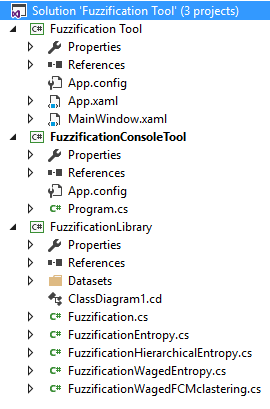
\includegraphics[width=0.35\textwidth]{obrazky/program.PNG}
\centering
\caption{Štruktúra projektu pre nástroj Fuzzy Tool} 
\label{fig:structure}
\end{figure}


\section{Implementácia nástroja fuzzy tool}

Na spracovanie dátových množín som navrhla triedu \textit{DataSets}, ktorá bude mať potomkov pre každý jeden druh datasetu (DatasetHeart, DatasetIris...). Na fuzzifikovanie dát som navrhla hlavnú triedu \textit{Fuzzification}, ktorá má potomkov \textit{FuzzificationEntropy}, \textit{FuzzificationHierarchicalEntropy}, \textit{FuzzificationWagedEntropy} a \textit{FuzzificationWagedFCMclastering}. V triede \textit{Fuzzification} budem využívať konkrétnu inštanciu DataSets. Na UML diagrame č.  \ref{fig:pohlad} sú zobrazené triedy s metódami a atribútmi a ich závislosti. 

\begin{figure}[ht]
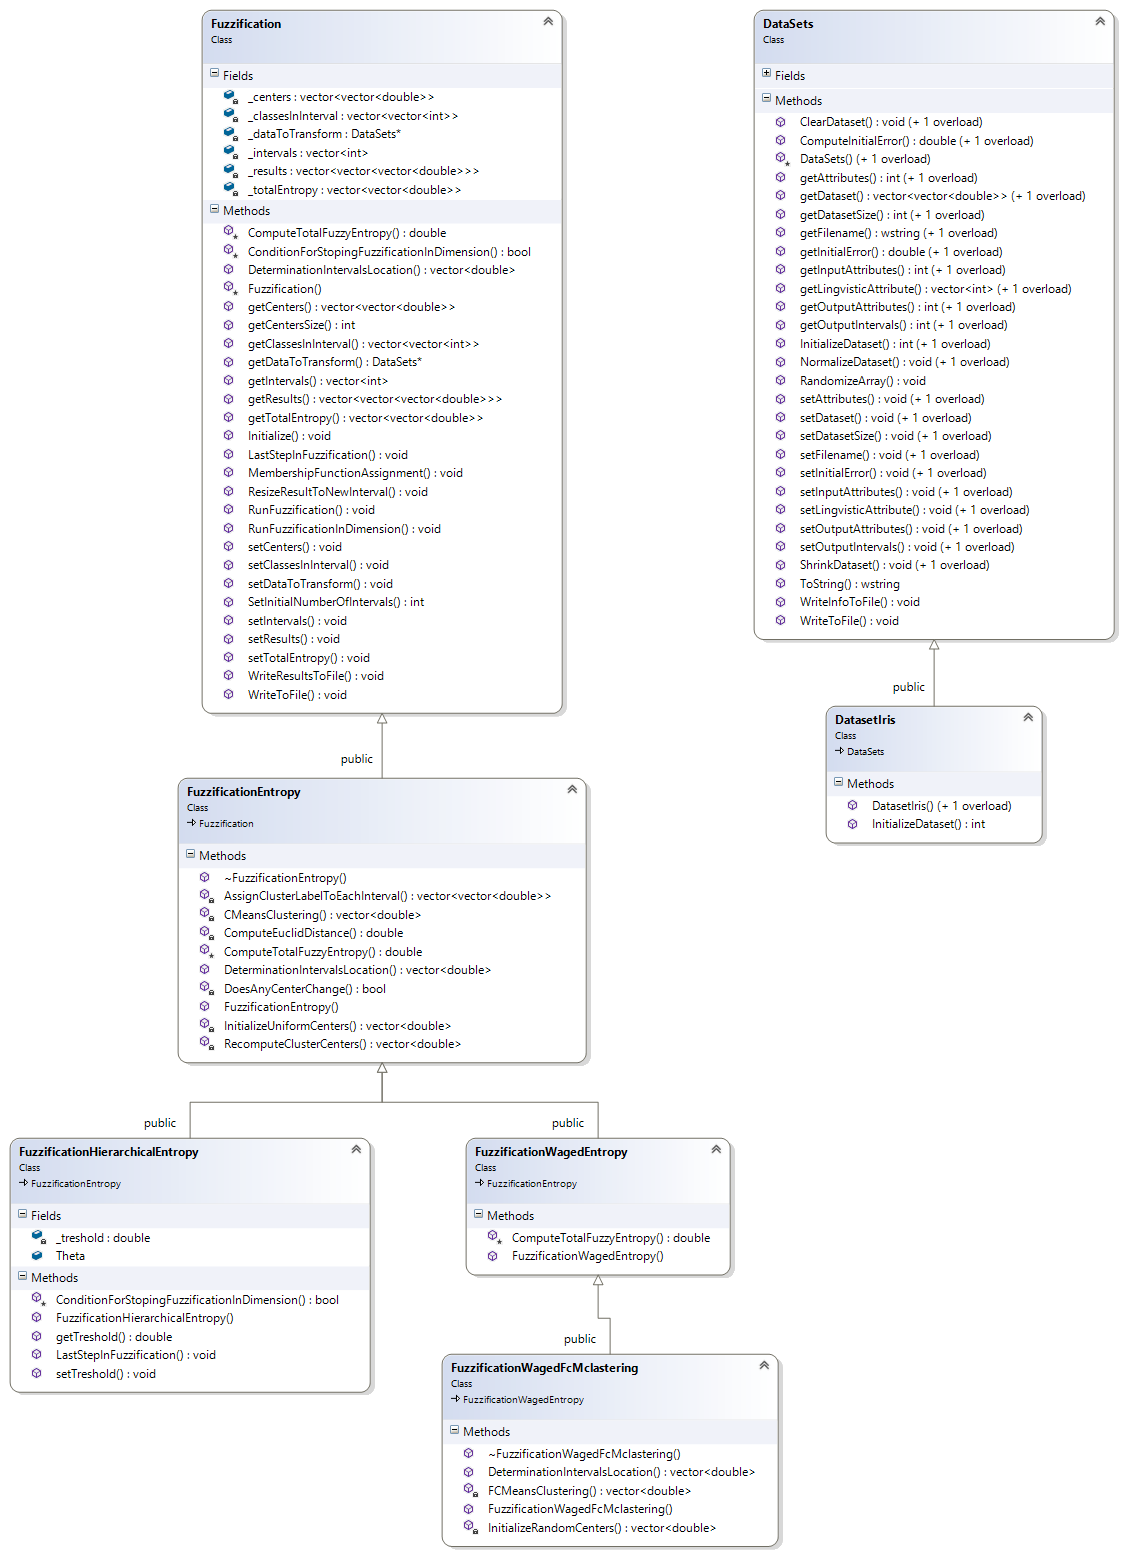
\includegraphics[width=0.95\textwidth]{obrazky/umldiagramcplusplus.png}
\centering
\caption{Diagram tried v C++} 
\label{fig:pohlad}
\end{figure}



Na obrázku číslo  \ref{fig:pohlad} je zobrazený diagram tried implementovaného fuzzification nástroja. Jednotlivé triedy a funkcionalitu opíšem v nasledujúcej časti. 

\subsection{Množiny dát - Datasets}

Na zadefinovanie vlastností súboru dát som použila nasledovné properties (v C++ get metódy): 
\begin{itemize}
\item \textit{Attributes} - počet vstupných a výstupných atribútov v dátovom súbore. 
\item \textit{InputAttributes} - počet vstupných atribútov v dátovom súbore. 
\item \textit{OutputAttributes} - počet výstupných atribútov, hodnota je 1. 
\item \textit{OutputIntervals} - počet intervalov výstupného parametra. 
\item \textit{LingvisticAttribute} - hodnoty lingvistického atribútu.
\item \textit{DatasetSize} - počet všetkých prvkov v dátovej množine. 
\item \textit{Filename} - názov vstupného súboru. 
\item \textit{InitialError} - počiatočná chyba, ktorá je vypočítaná po načítaní súboru. 
\item \textit{Dataset} - normalizované hodnoty datasetu v intervale $<0,1>$. 
\end{itemize}

Medzi hlavnú funkcionalitu triedy patrí metóda \textit{InitializeDataset}, ktorá je abstraktná a je prekrytá v jej potomkoch. Metóda vykonáva načítanie dát zo súboru, normalizovanie súboru a vypočítanie počiatočnej chyby. 

Potomkovia využívajú metódy triedy \textit{DataSets} a to sú tieto: 
\begin{itemize}
\item \textit{ClearDatasets} - vymazanie údajov. 
\item \textit{ComputeInitialError} - vypočítanie počiatočnej 
\item \textit{NormalizeDataset} - normalizácia dát do intervalu od nula po jedna.
\item \textit{RandomizeArray} - náhodne poprehadzuje poradie dát v dátovej množine.
\item \textit{ShrinkDataset} - zmenší dáta o zadané percento.
\item \textit{ToString} - všetky informácie v reťazci. 
\item \textit{WriteInfoToFile} - vypísanie podrobných informácií o datasete do súbora so zadaným názvom. 
\item \textit{WriteToFile} - vypísanie normovanej dátovej množiny do súboru. 
\end{itemize}

Diagram tried potomkov Datasetu je znázornený na obrázku č.\ref{fig:umldiagramdatasetou}  
\begin{figure}[ht!]
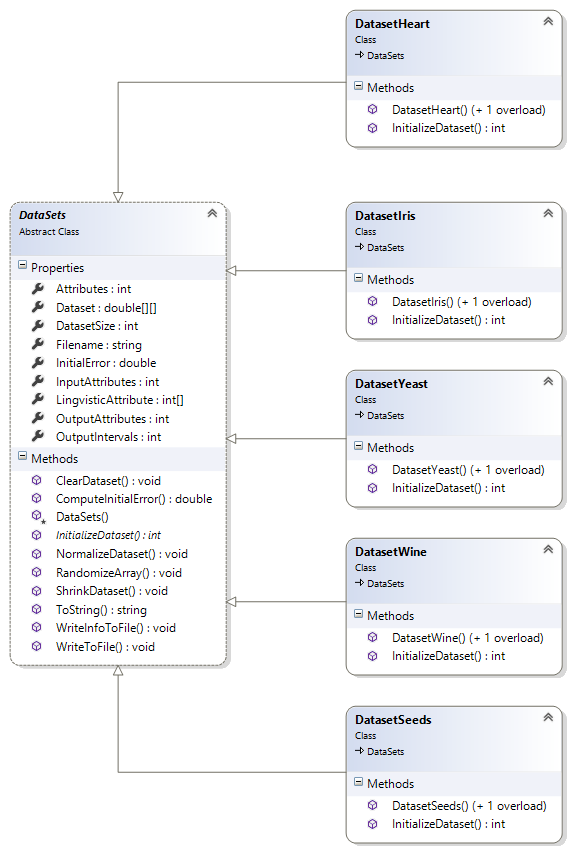
\includegraphics[width=0.85\textwidth]{obrazky/umldatasetov.png}
\centering
\caption{Diagram tried potomkov Datasetu } 
\label{fig:umldiagramdatasetou}
\end{figure}


\subsubsection{Spracovanie dát}
Inicializácia dát sa vykonáva vytvorením inštancie potomka textit{DataSets}. 
Táto inštancia je parametrom konštruktora abstraktnej triedy \textit{Fuzzification}, kde sa inicializuje do atribútu \textit{DataToTransform}. \textit{Centers} sú centrá všetkých atribútov dát v intervaloch.
Počty intervalov pre jednotlivé dimenzie sú v poli \textit{Intervals}. Výsledná množina fuzzifikovaných dát sa nachádza v poli \textit{Results}. Celková entropia pre jednotlivé intervaly je v poli \textit{TotalEntropy}. 

\textit{Fuzzification} trieda má zadefinovanú metódu \textit{Initialize}, v ktorej inicializuje všetky atribúty na defaulné hodnoty. \textit{RunFuzzification} je najdôležitejšia metóda triedy, pretože v nej sa spúšta celý proces transformácie numerických hodnôt na lingvistické. V tejto metóde sa inicializuje dátová množina, a pre všetky lingvistické atribúty sa nainicializuje ich hodnota do vopred určených intervalov. Následne sa pre všetky atribúty, ktoré nie sú lingvistické spustí proces transformácie reálnych dát na lingvistické. Pre každú dimenziu (t.j. atribút) sa vykoná metóda \textit{RunFuzzificationInDimension}. 
\begin{algorithm}[ht!]
\caption{Algoritmus \textit{RunFuzzificationInDimension} vykonáva nasledovné kroky:}
\label{runFuzzification}
\begin{algorithmic}
\STATE int interval = SetInitialNumberOfIntervals(dimension);
\STATE TotalEntropy[dimension][i] = 99999999999;
\STATE bool condition = false;
\WHILE {(!condition)}
\STATE ResizeResultToNewInterval(dimension, interval);
\STATE Centers[dimension] = DeterminationLocation(dimension, intervals);
\STATE MembershipFunctionAssignment(dimension, interval);
\STATE TotalEntropy[dimension][interval] = ComputeEntropy(dimension);
\STATE condition = ConditionForStoping(dimension,  TotalEntropy[dimension][interval], TotalEntropy[dimension][interval - 1]);  
\STATE  interval++;
\ENDWHILE
\STATE LastStepInFuzzification(dimension, interval);
\end{algorithmic}
\end{algorithm}

Na určenie polôh jednotlivých stredov intervalov je použitá abstraktná metóda. V prípade potomka \textit{FuzzificationEntropy} je počítaná klasickým K-Means algoritmom, a u potomka \textit{FuzzificationWagedFCMclastering} je pomocou algoritmu FCM. 

\textit{MembershipFunctionAssignment} je virtuálna metóda určená na výpočet hodnôt príslušností dát v určitom intervale.
 
Metóda na výpočet celkovej funkcie je abstraktná a v prípade potomka \textit{FuzzificationEntropy} sa vypočíta celková a pri potomkovi \textit{FuzzificationWagedEntropy} vážená entropia. 

V metóde \textit{LastStepInFuzzification} sa zníži počet intervalov a prepočítajú sa centrá a hodnoty funkcie príslušnosti. V prípade potomka \textit{FuzzificationHierarchicalEntropy} sa prekryje daná metóda,aby sa neznížil počet intervalov o jedna v poslednom kroku fuzzifikácie. 

Na zápis výsledkov a informácií o priebehu fuzzifikácie sú použité metódy WriteToFile, a WriteResultsToFile. 

Vzťahy a prepojenia jednotlivých potomkov triedy sú znázornené na obrázku č. \ref{fig:umlalgoritmov}.

\begin{figure}[ht]
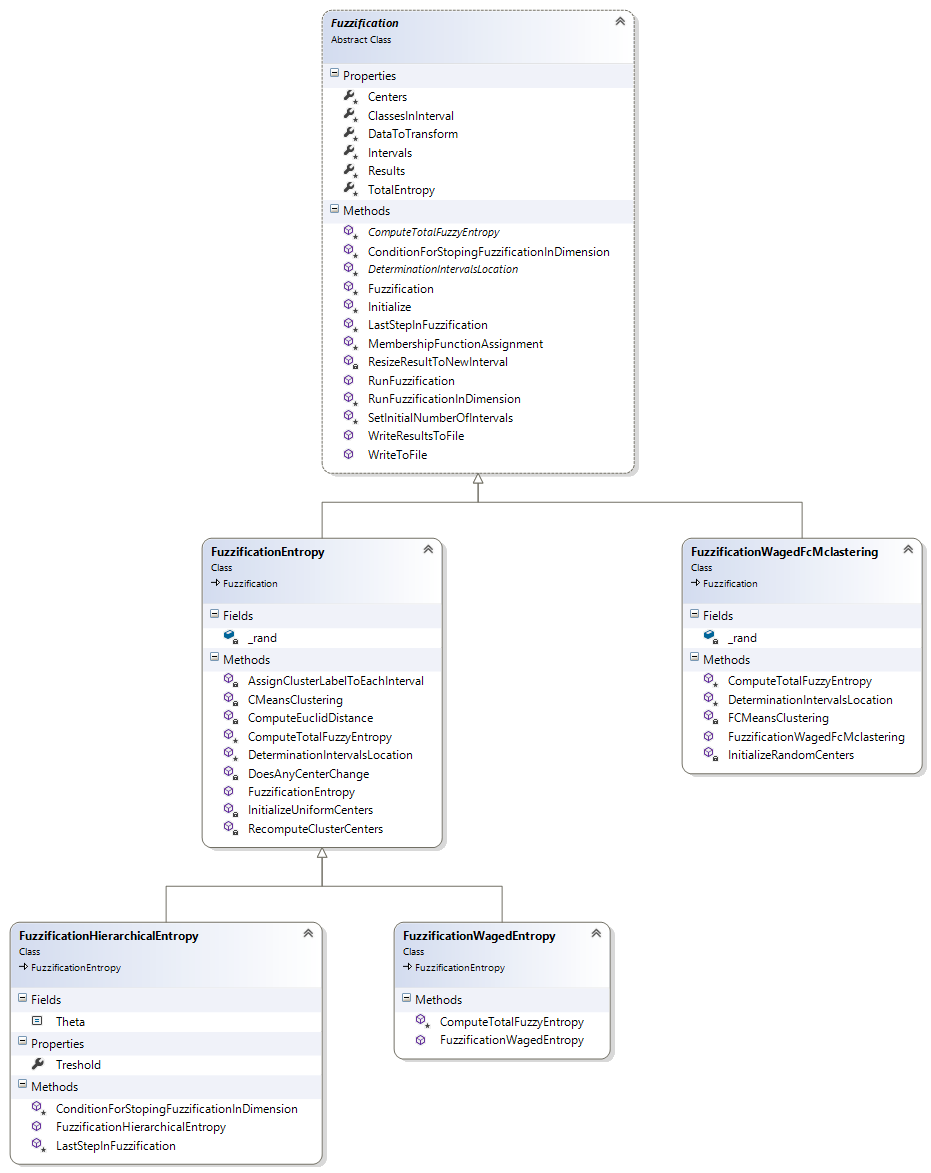
\includegraphics[width=0.95\textwidth]{obrazky/umlalgoritmov.png}
\centering
\caption{Diagram tried potomkov Datasetu } 
\label{fig:umlalgoritmov}
\end{figure}

\section{Ovládanie nástroja používateľom}

\subsection{Vstupné údaje programu}

Forma vstupných dát je vopred definovaná (dáta sú oddelené, buď čiarkov alebo iným oddeľovačom). Dáta, ktoré sa majú fuzzifikovať sú v priečinku spolu s programom. 

\subsection{Užívateľská príručka}
Ovládanie nástroja sa skladá z nasledujúcich krokov: 
\begin{enumerate}
\item Užívateľ spustí aplikáciu. Zobrazí sa mu menu, kde vyberie dátovú množinu a algoritmus fuzzifikácie. Menu konzolovej aplikácie je zobrazené na obrázku č. \ref{fig:konzolova_aplikaci} a menu grafického rozhrania je na obrázku č. \ref{fig:guivstupnemenu}. 

\begin{figure}[hp!]
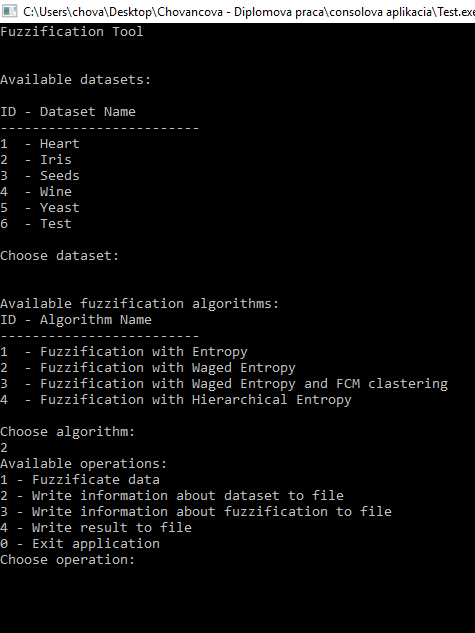
\includegraphics[]{obrazky/konzolova_aplikacia_-_vyberr_operacie.PNG}
\centering
\caption{Vstupné menu konzolovej aplikácie } 
\label{fig:konzolova_aplikaci}
\end{figure}

\begin{figure}[hp!]
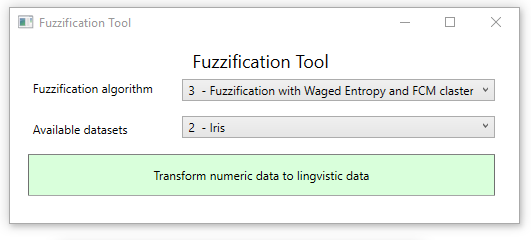
\includegraphics[]{obrazky/vyber_datasetu_a_algoritmu.PNG}
\centering
\caption{Vstupné menu grafického rozhrania } 
\label{fig:guivstupnemenu}
\end{figure}

\item Spustenie fuzzifikácie sa vykoná zadaním čísla jeden, a v prípade grafického rozhrania je to stlačenie tlačidla na fuzzifikovanie dát. 
\item Čakanie na výsledky. V prípade konzolovej aplikácie sa zobrazí aktuálna hodnota celkovej fuzzy entropie a počet tried v danom intervale pre konkrétny atribút.  
\item Úspešne fuzzifikovanie dát. Užívateľ je upozornení o úspešnom ale aj neúspešnom vykonaní fuzzifikácie. V prípade konzolovej aplikácie je to správa vypísaná na konzolu, a pre grafické rozhranie je to vyskakovacie okno, ktoré je znázornené na obrázku č. \ref{fig:guivstupnemenu2}. 

\begin{figure}[hp!]
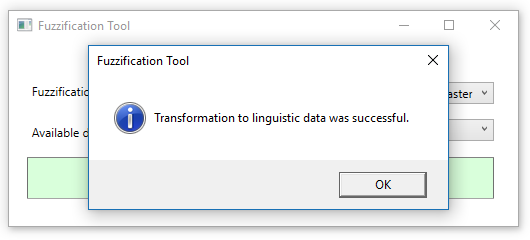
\includegraphics[]{obrazky/gui_-_po_fuzzifikovani.PNG}
\centering
\caption{Grafické rozhranie po úspešnom fuzzifikovaní dát} 
\label{fig:guivstupnemenu2}
\end{figure}

\item Ďalšie operácie. V prípade konzolovej aplikácie užívateľ zadá ďalšie dodatočné operácie. Výpis výsledkov do súboru (voľba 4), výpis informácií o dátovej množine (voľba 2) a podrobnejšie výsledky fuzzifikácie (voľba 3) do súboru. 
\item Súbory. Užívateľ nájde výsledné súbory v priečinku, ako je znázornené na obrázku č. \ref{fig:obsah_priecinka_po_fuzzifikacii}.

\begin{figure}[hp!]
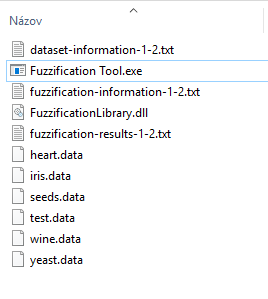
\includegraphics[]{obrazky/obsah_priecinka_po_fuzzifikacii.PNG}
\centering
\caption{ Príklad štruktúry priečinku po fuzzifikácií} 
\label{fig:obsah_priecinka_po_fuzzifikacii}
\end{figure}


\end{enumerate}


\subsection{Opis výstupných súborov programu}
\subsubsection{Informácie o vstupnom súbore}
V  súbore \textit{dataset-information} sú zobrazené základné informácie o súbore dát, ktoré boli fuzzifikované. Obsahuje počet dát, vstupných atribútov, výstupných atribútov, výstupných intervalov, počet intervalov lingvistických dát, názov súboru, počiatočnú chybu a normované dáta.   

\subsubsection{Výsledky fuzzifikácie}
Výsledky fuzzifikácie sú zapísané do súboru  \textit{fuzzification-results}. Obsahuje lingvistické dáta v rozsahu od nula po jedna, a súčet intervalu pre konkrétny atribút dáva hodnotu jedna. Príklad obsahu súboru je znázornený na obrázku č.\ref{fig:vysledky_subor}. 

\begin{figure}[hp!]
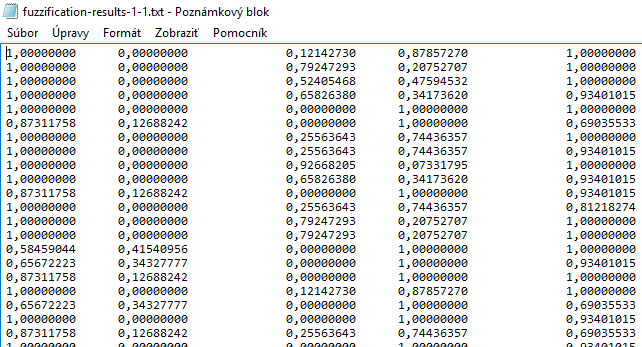
\includegraphics[width=0.85\textwidth]{obrazky/obsah_suboru_-_fuzzification-results.PNG}
\centering
\caption{Príklad obsahu súboru s výsledkami} 
\label{fig:vysledky_subor}
\end{figure}



\subsubsection{Podrobnejšie výsledky fuzzifikácie}
Podrobnejšie výsledky sú zapísané do súboru \textit{fuzzification-information}. Obsahuje údaje celkovej entropie pre jednotlivé dimenzie na každom intervale. Ďalej obsahuje počet intervalov pre každú dimensiu a ako aj lokáciu jednotlivých centier. V súbore sa nachádzajú aj počty výstupných tried čo sa nachádzajú na danom atribúte. Na konci súboru sú výsledky fuzzifikácie spolu s kontrolným súčtom jedna. Príklad obsahu súboru je znázornený na obrázku č. \ref{fig:vysledky_subor_dalsie}. 

\begin{figure}[hp!]
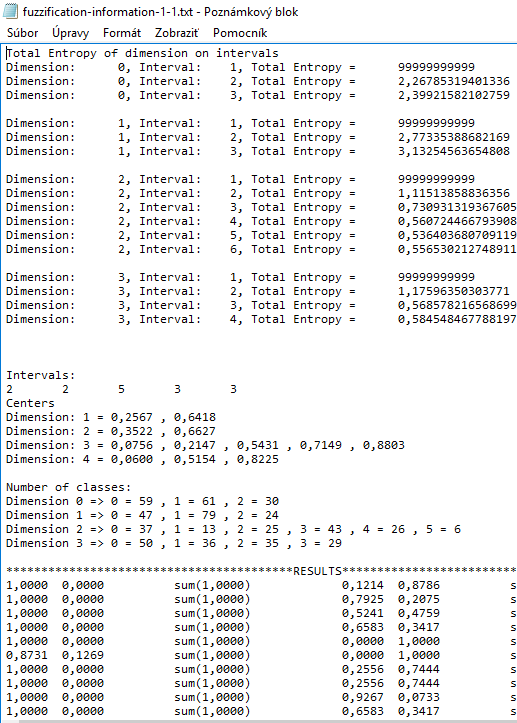
\includegraphics[width=0.85\textwidth]{obrazky/obsah_suboru_-_fuzzification-information.PNG}
\centering
\caption{Príklad obsahu súboru s podrobnejšími výsledkami} 
\label{fig:vysledky_subor_dalsie}
\end{figure}



